% !TeX spellcheck = en_US
% !TeX root = ../Tom_Sandmann-master_thesis
\section{Online Template Attack}  \label{sec: Online Template Attack}
In \cite{batina2014online}, a variation of template attacks called \emph{Online Template Attacks} (OTAs) is introduced.
Template attacks are a form of SCAs with a \emph{modus operandi} called \emph{Vertical}.
In these attacks, the implementation under attack is executed several times, such that power traces can be acquired for each of these executions.
Whether these executions use the same input or not depends on whether a simple or advanced SCA is performed.
Besides Vertical SCAs, we also have SCAs with a \emph{modus operandi} called \emph{Horizontal}.
In these attacks, only a single execution is necessary and different (Horizontal) data or computations are considered when attacking the implementation.
The differences between these \emph{modus operandi} of SCAs can be seen in \Cref{fig: vertical_and_horizontal_sca}.
%
\begin{figure}
	\centering
	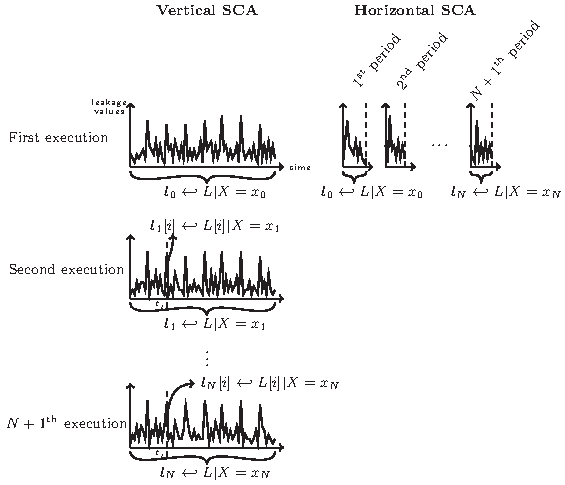
\includegraphics[scale=1.2]{vertical_and_horizontal_sca}
	\captionof{figure}{Visualization of Vertical and Horizontal SCAs (taken from \cite{bauer2013horizontal}).
	A realization of random variable $X$ is referred to as the corresponding lower-case letter $x$.
	A power trace $l_i$ for a given input $x_i$ is denoted as $l_i \hookleftarrow L \mid X = x_i $ (this notation sums up the event of a sample of observations of $L$ under the input $x_i$).
	}
	\label{fig: vertical_and_horizontal_sca}
\end{figure}
%
An OTA combines these two different approaches to SCAs. 
The attack works by acquiring one target trace from the device under attack.
Patterns of certain operations from this target trace are then compared to templates obtained from the attacker's device (which is a similar device running the same implementation).
Thus, an attacker requires only one \emph{target trace} from the \emph{target device}.
Only a single template trace per key-bit is necessary, which is obtained from the device of the attacker.
OTAs can be used to attack the secret scalar used in a scalar multiplication algorithm.
In practice, OTAs make the following assumptions about the attacker \cite{batina2014online, dugardin2016dismantling}:
%
\begin{itemize}
	\item The attacker knows the input point $\mathcal{P}$ that belongs to the trace of the target device;
	\item The attacker knows the implementation of the scalar multiplication algorithm and can compute intermediate values of this algorithm;
	\item The attacker can choose the input point on a device similar to the target device.
\end{itemize}
%
For the attack to work, at least one assignment in the exponentiation algorithm must be dependent on the value of particular scalar bit(s). 
However, there should not be any branches with key-dependent computations.
We now give a global overview of how an OTA works:
%
\begin{itemize}
	\item First, the attacker obtains a target trace with input point $\mathcal{P}$ from the target device;
	\item The attacker now obtains the template traces with input points $[m]P$ for $m \in \mathbb{Z}$.
	 This is done for multiples of the point $\mathcal{P}$, for example $2\mathcal{P}$ or $3\mathcal{P}$;
	 \item The attacker now compares the correlations between the target trace and each pair of template traces.
	 The one with the highest correlation is the one most likely to be correct.
\end{itemize}
%

\subsection{Creating the templates}
In \cite{batina2014online}, several examples are shown on how an OTA works for different scalar multiplication algorithms.
Consider the left-to-right double-and-add always algorithm shown in \Cref{Left-to-right double-and-add-always}.
%
\begin{algorithm}
	\algorithmicrequire $\bm{\mathcal{P}}$, $k = (1, k_{x-2}, \ldots, k_0)_2$. \\
	\algorithmicensure $\bm{Q} = k \cdot \bm{\mathcal{P}}$.
	%	
	\begin{algorithmic}[1]
		\State $\bm{R}_0 \gets \bm{\mathcal{P}}$ 
		\For{$i = x - 2$ \textbf{to} $0$}
			\State $\bm{R}_0 \gets 2 \bm{R}_0$
			\State $\bm{R}_1 \gets \bm{R}_0 + \bm{\mathcal{P}}$
			\State $\bm{R}_0 \gets \bm{R}_{k_i}$ \Comment{Depending on the bit value of $k_i$, $\bm{R}_0$ either takes the value $\bm{R}_0$ or $\bm{R}_1$}
		\EndFor
		\State \textbf{Return} $\bm{R}_0$
	\end{algorithmic}
	%
	\captionof{algorithm}{Left-to-right double-and-add-always algorithm \cite{batina2014online}.}
	\label{Left-to-right double-and-add-always}
\end{algorithm}
%
The algorithm assumes that the most-significant bit of the scalar $k$ is 1 (i.e. $k_\text{MSB} = 1$).
We now describe how an OTA can be applied in the case of \Cref{Left-to-right double-and-add-always}.
It is assumed that the first bit of the scalar is $1$.
However, if we take a look at the `for loop' in \Cref{Left-to-right double-and-add-always}, we see that this bit is not used.
Therefore, we assume that the first iteration of this algorithm (which involves a point doubling and addition) is done with the neutral element of the curve.
Thus, execution of the first iteration will yield the point $\mathcal{P}$.
If we now consider the second iteration (the operations that correspond to $k_\text{MSB} - 1$), we can verify that the expected outputs of this iteration are either $2 \mathcal{P}$ or $3 \mathcal{P}$ (depending on the value of $k_{\text{MSB} - 1}$). 
We now know that in the next iteration (i.e. the operations belonging to key-bit $k_{\text{MSB} - 2}$), a doubling of either $2 \mathcal{P}$ or $3 \mathcal{P}$ will be performed.
On our copy of the same device, we can now execute the algorithm with input point $2 \mathcal{P}$ or $3 \mathcal{P}$. This gives us a trace of the corresponding doubling operations.
Thus we can match the trace of the doubling operation in the ${(i + 1)}^\mathrm{th}$ iteration of the target trace with the appropriate template trace to attack the key bit used in the $i^\mathrm{th}$ iteration:
%
\begin{itemize}
	\item  If $k_{\text{MSB} - 1} = 0$, then the output of the second iteration is $2 \mathcal{P}$. The template trace for $2\mathcal{P}$ (obtained from the iteration involving $k_{\text{MSB} - 2}$) will now give a higher correlation with the target trace than the template trace for $3\mathcal{P}$.
	
	\item If $k_{\text{MSB} - 1} = 1$, then the output of the second iteration is $3 \mathcal{P}$. The template trace for $3\mathcal{P}$ (obtained from the iteration involving $k_{\text{MSB} - 2}$) will now give a higher correlation with the target trace than the template trace for $2\mathcal{P}$.
\end{itemize}
%
In this way, we can iteratively attack and retrieve all of the key bits used.
Note that when we calculate the correlation of the template trace with the target trace, we compare them only at the \emph{suitable} parts of the traces. 
These are the places at which the key-bit related assignments take place.
To determine the most likely key-bit, we compute the correlations with the target trace and the template traces, which in the second iteration would be $2\mathcal{P}$ and $3\mathcal{P}$. 
We consider the template trace that gives the highest correlation value as the one with the right key guess.
We repeat this procedure to find the key-bit for $k_{\text{MSB} - 2}$: we correlate the templates for $4\mathcal{P}$ and $5\mathcal{P}$ with the target trace if we guessed that $k_\text{MSB} - 1 = 0$.
Otherwise, we would correlate using the templates $6\mathcal{P}$ and $7\mathcal{P}$.
Again, the template that gives the highest correlation with the target trace is the most likely one to be correct.
An example of attacking the first two bits of a secret scalar $k$ with respect to \Cref{Left-to-right double-and-add-always} can be seen in \Cref{table: OTA example visualization}.
%
\begin{table}
	\centering
	%
	% Iteration 2 example
	%
	\subfloat[Attacking the second-most significant key bit $K_{\text{MSB} - 1}$. $\operatorname{D}$ and $\operatorname{A}$ stand for the doubling and addition operation respectively as performed in \Cref{Left-to-right double-and-add-always}. Depending on the correlation of the output of the operations performed using the key-bit $K_{\text{MSB} - 1}$ and the corresponding template traces (in this case the template trace $\operatorname{D}(2 \mathcal{P})$), we determine the most likely value for $K_{\text{MSB} - 1}$. In this iteration, we assume that the template for $\operatorname{D}(2 \mathcal{P})$ gives the highest correlation with the target trace.]{
	%
	\begin{tabular}{*7c}
		\toprule
		& \multicolumn{2}{c}{$K_{\text{MSB}} = 1$}  & \multicolumn{2}{c}{$K_{\text{MSB} - 1} \in \{\textcolor{red}{0}, \textcolor{blue}{1}\}$}  & \multicolumn{2}{c}{$K_{\text{MSB} - 2}$} \\
		\midrule
		\textbf{Target Trace} & $\operatorname{D}(\mathcal{O})$ & $\operatorname{A}(\mathcal{O}, \mathcal{P})$ & $\operatorname{D}(\mathcal{P})$ & $\operatorname{A}(2\mathcal{P}, \mathcal{P})$ & $\textcolor{red}{\operatorname{D}(2\mathcal{P})}$ \emph{or} $\textcolor{blue}{\operatorname{D}(3\mathcal{P})} $ & \\
		%
		\multicolumn{7}{c}{} \\
		%
		\textbf{Template Trace of $2 \mathcal{P}$}  & $\operatorname{D}(\mathcal{O})$ & $\operatorname{A}(\mathcal{O}, 2\mathcal{P})$ & \cellcolor{red!20} $\operatorname{D}(2\mathcal{P})$ & $\operatorname{A}(4\mathcal{P}, 2\mathcal{P})$ &  &  \\
		\bottomrule
	\end{tabular}
	%
	\label{table: OTA template matching iteration 2}
	}
	\vfill
	%
	% Iteration 3 example
	%
	\subfloat[Attacking the third-most significant key bit $K_{\text{MSB} - 2}$. 
	Depending on the correlation of the output of the operations performed using the key-bit $K_{\text{MSB} - 2}$ and the corresponding template traces (in this case the template trace $\operatorname{D}(4 \mathcal{P})$), we determine the most likely value for $K_{\text{MSB} - 2}$.]{
		% TODO manually scaled the textwidth, otherwise tablew would still be to wide
		\begin{adjustbox}{max width=.98\textwidth}
			%
			\begin{tabular}{*9c}
				\toprule
				& \multicolumn{2}{c}{$K_{\text{MSB}} = 1$}  & \multicolumn{2}{c}{$K_{\text{MSB} - 1} = 0$}  & \multicolumn{2}{c}{$K_{\text{MSB} - 2} \in \{\textcolor{red}{0}, \textcolor{blue}{1}\}$} & \multicolumn{2}{c}{$K_{\text{MSB} - 3}$} \\
				\midrule
				\textbf{Target Trace} & $\operatorname{D}(\mathcal{O})$ & $\operatorname{A}(\mathcal{O}, \mathcal{P})$ & $\operatorname{D}(\mathcal{P})$ & $\operatorname{A}(2\mathcal{P}, \mathcal{P})$ &
				$\operatorname{D}(2\mathcal{P})$ & $\operatorname{A}(4\mathcal{P}, \mathcal{P})$ & $\textcolor{red}{\operatorname{D}(4\mathcal{P})}$ \emph{or} $\textcolor{blue}{\operatorname{D}(5\mathcal{P})} $ & \\
				%
				\multicolumn{9}{c}{} \\
				%
				\textbf{Template Trace of $4 \mathcal{P}$}  & $\operatorname{D}(\mathcal{O})$ & $\operatorname{A}(\mathcal{O}, 4\mathcal{P})$ & \cellcolor{red!20} $\operatorname{D}(4\mathcal{P})$ & $\operatorname{A}(8\mathcal{P}, 4\mathcal{P})$ &  & & & \\
				\bottomrule
			\end{tabular}
		%
		\end{adjustbox}
		\label{table: OTA template matching iteration 3}
	}
	%
	\captionof{figure}{Visualization of the first two iterations of the OTA applied to \Cref{Left-to-right double-and-add-always} (tables based on examples shown in \cite{dugardin2016dismantling}).}
	\label{table: OTA example visualization}
\end{table}
%

\subsection{Matching the templates}
As mentioned previously, template matching is only performed with parts of the power trace at which the key-bit related assignments take place.
To calculate the correlation between a template and target trace such that we can distinguish the right hypothesis on the current bit under attack, we can make use of the Pearson correlation coefficient. 
The Pearson correlation coefficient is defined as follows:
%
\begin{equation*}
\rho(X, Y) = \frac{\operatorname{cov}(X, Y)}{\sigma_X \sigma_Y}
\end{equation*}
%
where $\operatorname{cov}$ is the covariance, $\sigma_X$ is the standard deviation of $X$ and $\sigma_Y$ is the standard deviation of $Y$.
$X$ and $Y$ would in this case be the template and target trace (in any order).